\documentclass[a4paper, 11pt]{article}
\usepackage{amsmath}
\usepackage{amsfonts}
\usepackage{amssymb}
\usepackage{caratula}
\usepackage[spanish, activeacute]{babel}
\usepackage[usenames,dvipsnames]{color}
\usepackage[width=15.5cm, left=3cm, top=2.5cm, height= 24.5cm]{geometry}
\usepackage{graphicx}
\usepackage[utf8]{inputenc}
\usepackage{listings}
\usepackage[all]{xy}
\usepackage{multicol}
\usepackage{subfig}

\usepackage{cancel}
\usepackage{float}
\usepackage{xcolor}
\usepackage{color,hyperref}

\usepackage{multirow} % para las tablas


%%%%%%%%%%%%%% ALGUNAS MACROS %%%%%%%%%%%%%%
% For \url{SOME_URL}, links SOME_URL to the url SOME_URL
\providecommand*\url[1]{\href{#1}{#1}}

% Same as above, but pretty-prints SOME_URL in teletype fixed-width font
\renewcommand*\url[1]{\href{#1}{\texttt{#1}}}

% Comando para poner el simbolo de Reales
\newcommand{\real}{\hbox{\bf R}}

\providecommand*\code[1]{\texttt{#1}}

%uso: \ponerGrafico{file}{caption}{scale}{label}
\newcommand{\ponerGrafico}[4]
{\begin{figure}[H]
	\centering
	\subfloat{\includegraphics[scale=#3]{#1}}
	\caption{#2} \label{fig:#4}
\end{figure}
}

%\renewcommand{\algorithmiccomment}[1]{\hfill #1}

%%%%%%%%%%%%%%%%%%%%%%%%%%%%%%%%%%%%%%%%%%%%

\materia{Ingeniería de Software II}

\titulo{Enviá AULA al 2020}
%\fecha{fecha de entrega}
%\grupo{Nro grupo}
\integrante{Agustina Ciraco}{630/06}{agusciraco@gmail.com}
\integrante{Alejandro Rebecchi}{15/10}{alejandrorebecchi@gmail.com}
\integrante{Maria Lara Gauder}{27/10}{marialaraa@gmail.com}
\integrante{Martin Heredia}{146/11}{martin.herediaf@gmail.com}

\include{templates}

\begin{document}
\pagestyle{myheadings}
\maketitle
%\markboth{Nombre materia}{Nombre TP}

\thispagestyle{empty}
\tableofcontents

%\setcounter{section}{-1}
\newpage

\section{Introducción}
En este proyecto define el desarrollo e implementación de un programa denominado "Aula al 2020". El mismo será utilizado en los colegios para mejorar el rendimiento de los alumnos antes diversas situaciones. 

El sistema permitirá al docente notificar a los alumnos de una fecha de un examen e ir dando aviso paulatino del mismo. En el caso de un alumno más flojo, podrá enviarle mensajes desde una determinado tiempo anterior a la prueba, indicándole qué debería ir haciendo. Por el otro lado, en el caso de un alumno responsable, podría simplemente avisarle un tiempo antes de la fecha del examen. 

El sistema podrá también ser utilizado para eventos que no pertenecen al aula. Sería como ejemplo, el de traer la autorización a la visita de un comedor junto con un alimento no perecedero. El personal correspondiente a la Secretaría o Dirección del colegio podrán enviarle mensajes a los alumnos y padres de los mismos con recordatorios de la excursión y de lo que deben traer a la misma.

En el sistema se permitirá la creación de campañas asociadas a eventos, y campañas asociadas entre si. Las campañas representan las acciones que se realizan para un evento en especial. Puede existir varias campañas relacionadas a un único evento, como en el ejemplo del examen dado previamente (dos secuencias diferentes de mensajes para dos tipos de alumnos). Las campañas permitirán ir agregando los mensajes que desean ser enviados en una determinada fecha. 

Además, para poder observar la eficiencia de la campaña creada y si fue correctamente administrada, una vez finalizado la fecha del evento se podrán cargar los resultados obtenidos para cada campaña y así observar las mejoras o empeoramiento de aplicarla. 

El docente únicamente podrá tener acceso a todas aquellas campañas o eventos que haya creado. A si mismo, solo podrá acceder a los alumnos y padres que correspondan a la clase que tiene dicta. Alguien perteneciente a la Secretaría o Dirección serán los encargados de gestionar los permisos necesarios para el docente hacia los alumnos y sus padres. 

Existirán únicamente dos ¿ROLES?, el del Docente, que es quien dicta las clases, y el del personal de la Secretaría (secretario, preceptor, etc) o la Dirección (director, vicedirector). De esta manera, a continuación se presentan los items del Product Backlog que fueron definidos por el equipo a partir de los requerimientos del cliente. Luego, los mismos fueron evaluados para definir el valor de cada storie. Fue un proceso de decisión y debate para poder estar de acuerdo en la cantidad de puntos a asignar a cada una. Además se presenta el esfuerzo designado a cada storie. En la siguiente sección, se definen las tareas que se deben desarrollar para cada storie y su criterio de aceptación correspondiente. 

\newpage
\section{Product Backlog}

\begin{table}[H]
\centering
\begin{tabular}{ | p{1cm} | p{10cm} | p{1cm} | p{1cm} |}
\hline
ID & User Story & Effort & Value \\ \hline \hline
1 & Como Docente quiero enviar un SMS con un determinado contenido a ciertos alumnos o padres asignados a mi, en una fecha definida para poder dar un aviso o comunicar algo. & 8 & 13 \\ \hline


2 & Como Docente quiero ingresar al sistema utilizando un usuario y contraseña propio para poder acceder al mismo con los permisos que me corresponda. & 3 & 8 \\ \hline


3 & Como personal de la Secretaría o la Dirección debo poder dar de alta a un Docente. & 3 & 3 \\ \hline


4 & Como Docente quiero poder editar a las campañas y los eventos que yo generé para cambiar la fecha del evento, el título de alguno, entre otras cosas. & 3 & 3 \\ \hline


5 & Como personal de la Secretaría o Dirección quiero dar de alta una campaña y asociarla a un evento para poder comenzar un proceso de envío de mensajes. & 1 & 3 \\ \hline


6 & Como Docente quiero poder ver los mensajes que ya fueron enviados y los que no para poder corroborrar el correcto funcionamiento del mismo. & 1 & 1 \\ \hline


7 & Como personal de la Secretaría o Dirección quiero poder ver la asociación de una campaña a otras para poder tener una visualización clara de las relaciones definidas previamente. & 2 & 2 \\ \hline


8 & Como personal de la Secretaría o Dirección quiero poder visualizar y modificar los datos de alumnos y padres/tutores para que, en el caso de modificarlos, se actualicen en el sistema. & 3 & 3\\ \hline


9 & Como Docente o personal de la Dirección o Secretaría quiero poder cargar los resultados obtenidos en una campaña para poder evaluar la eficacia del mismo.  & 5 & 5 \\ \hline


10 & Como Docente o personal de la Dirección o Secretaría quiero dar de alta una campaña para comenzar el proceso de envío de mensajes. & 5 & 8 \\ \hline


11 & Como personal de la Secretaría o Dirección quiero poder agregar un alumno/padre al sistema para que se pueda enviarle, luego, los SMS que requiera. & 5 & 5  \\ \hline


12 & Como personal de Secretaría quiero poder asociar un alumno a un Docente para que este último pueda acceder a los datos que requiera del mismo. & 5 & 5\\ \hline


13 & Como Docente quiero poder obtener una comparación entre los resultados de dos campañas para poder, luego, evaluar la eficiencia de la campaña implementada. & 8 & 5\\ \hline


14 & Como personal de la Dirección o Secretaría quiero ingresar al sistema utilizando un usuario y contraseña propio para poder acceder al mismo con los permisos que me corresponda. & 8 & 3 \\ \hline


15 & Como Docente quiero dar de alta una campaña y asociarla a un evento para poder comenzar un proceso de envío de mensajes. & 3 & 5 \\ \hline

\end{tabular}
\end{table}

\newpage

\begin{table}[H]
\centering
\begin{tabular}{ | p{1cm} | p{10cm} | p{1cm} | p{1cm} |}
\hline
ID & User Story & Effort & Value \\ \hline \hline

16 & Como personal de la Secretaría o de la Dirección quiero poder editar a las campañas y los eventos para cambiar la fecha del evento, el título de alguno, entre otras cosas. & 3 & 3\\ \hline


17 & Como Docente quiero poder tener acceso a las campañas y los eventos que yo generé para poder observar toda la información de los mismos. & 5 & 3\\ \hline


18 & Como personal de la Secretaría o de la Dirección quiero tener acceso a todas las campañas y los eventos para poder observar las acciones realizadas. & 3 & 3 \\ \hline


19 & Como Docente quiero poder ver la asociación de una campaña a otras para poder tener una visualización clara de las relaciones definidas previamente. & 3 & 2 \\ \hline


20 & Como Docente quiero poder acceder a las campañas que yo cree para cargar los resultados de la misma para luego generar estadísticas de los mismos. & 5 & 5 \\ \hline


21 & Como personal de la Secretaría o de la Dirección quiero poder enviar un SMS con un determinado contenido a ciertos alumnos o padres del colegio en una fecha definida para poder dar un aviso o comunicar algo. & 8 & 13 \\ \hline


22 & Como personal de la Secretaría o Dirección quiero poder ver los mensajes que ya fueron enviados y los que no para poder corroborar el correcto funcionamiento del mismo. & 1 & 1 \\ \hline


23 & Como personal de Secretaría o Dirección quiero poder obtener una comparación entre los resultados de dos campañas para poder, luego, evaluar la eficiencia de la campaña implementada. & 8 & 5\\ \hline

\end{tabular}
\end{table}

\section{Sprint backlog}
\begin{table}[H]
\centering
\begin{tabular}{ | p{0.5cm} | p{4cm} | p{5cm} | p{0.85cm} | p{5cm} | }
\hline
ID & User Story & Tareas & Horas & Criterio de aceptación \\
\hline \hline

1 & \multirow{4}{4cm}{Como Docente quiero enviar un SMS con un determinado contenido a ciertos alumnos o padres asignados a mi, en una fecha definida para poder dar un aviso o comunicar algo.} & Implementar un programa que se encargue de enviar los mensajes de texto de acuerdo a la fecha configurada. & 5 & \multirow{4}{5cm}{El usuario podrá enviar el sms sólo si están los  campos de destinatario, cuerpo del mensaje y fecha completados. En caso de que el Docente no complete correctamente los campos, entonces no se podrá enviar el mensaje de texto. El campo destinatario deberá indicar a que padres o alumnos se envían el mensaje, los mismos podrán ser únicamente los que pertenezcan a la clase que tienen a cargo. El cuerpo del mensaje contendrá el texto que se quiere enviar en el SMS y la fecha indicará el momento en que se desea enviar. El sistema almacenará si el mensaje se envió correctamente, sin necesidad de saber si le llegaron correctamente a los destinatarios.
Se almacenará la creación del mensaje de texto junto con sus características. 
En el momento que ocurra el día de la fecha indicada en el SMS, el mismo deberá enviarse a los destinatarios indicados. } \\[3.5cm] \cline{3-4} 
& & Desarrollar un sistema automático de registro del resultado del envío en la campaña. & 0,5 & \\[3.5cm] \cline{3-4} 
& & Crear modelo del mensaje. & 1 & \\[3.5cm] \cline{3-4} 
& & Asociar los mensajes a una campaña. & 1,5 & \\[3.5cm] \hline

\end{tabular}
\end{table}




\begin{table}[H]
\centering
\begin{tabular}{ | p{0.5cm} | p{4cm} | p{5cm} | p{0.85cm} | p{5cm} |}
\hline 
ID & User Story & Tareas & Horas & Criterio de aceptación \\ \hline \hline


2 & \multirow{3}{4cm}{Como Docente quiero ingresar al sistema utilizando un usuario y contraseña propio para poder acceder al mismo con los permisos que me corresponda.} & Crear interfaz para logearse y deslogearse. & 1 & \multirow{3}{5cm}{El formulario de ingreso no debe poder ser enviado sin completar usuario y contraseña. Se debe requerir reingresar los datos hasta que se ingrese una combinación de usuario y contraseña válidos. Sólo se debe poder acceder al formulario de inicio de sesión si no hay una sesión activa (y a ninguna otra cosa). Una vez iniciada la sesión, solo se deben aplicar las restricciones correspondientes al usuario que corresponde a los datos ingresados. Al desloguearse se debe destruir la sesión en curso.} \\[3.4cm] \cline{3-4}
& & Implementar el manejo de sesiones. & 7 & \\[3.4cm] \cline{3-4}
& & Implementar un validador de usuario y contraseña para el usuario Docente. & 2 & \\[3.4cm] \hline


3 & \multirow{3}{4cm}{Como personal de la Secretaría o la Dirección debo poder dar de alta a un Docente.} & Crear interfaz para crear el usuario del Docente. & 1 & \multirow{3}{5cm}{El docente será debidamente ingresado al sistema. Para poder ser ingresado al sistema se debió completar un formulario con los datos necesarios para ese usuario (Nombre, Apellido, DNI, observaciones). El usuario creado sea un Docente, entonces, tendrá permisos de acceso restringidos. } \\[2.5cm] \cline{3-4} 
& & Permitir la creación del usuario del Docente con la configuración dada. & 1 & \\[2.5cm] \cline{3-4}
& & Crear modelo del Docente. & 1 & \\[2.5cm] \hline

\end{tabular}
\end{table}




\begin{table}[H]
\centering
\begin{tabular}{ | p{0.5cm} | p{4cm} | p{5cm} | p{0.85cm} | p{5cm} |}
\hline 
ID & User Story & Tareas & Horas & Criterio de aceptación \\ \hline \hline


4 & \multirow{3}{4cm}{Como Docente quiero poder editar a las campañas y los eventos que yo generé para cambiar la fecha del evento, el título de alguno, entre otras cosas.} & Generar permisos que sean validados al editar las campañas y eventos por el usuario Docente. & 0,5 & \multirow{3}{4cm}{Al momento de querer editar las configuraciones u observarlas de las campañas, el Docente sólo podrá acceder a aquellas de las cuales fue creador. No podrá ver ni editar ninguna campaña de la cual no es owner. El Docente podrá modificar el título y/o la fecha del evento, siempre y cuando la fecha sea válida, es decir, no haya pasado aún.} \\[2.5cm] \cline{3-4}
& & Generar interfaz que permita modificar los datos de las campañas y los eventos. & 2 & \\[2.5cm] \cline{3-4}
& & Implementar proceso que modifique la información de las campañas o los eventos a partir de las nuevas configuraciones. & 1 & \\[2.5cm] \hline


5 & \multirow{3}{4cm}{Como personal de la Secretaría o Dirección quiero dar de alta una campaña y asociarla a un evento para poder comenzar un proceso de envío de mensajes.} & Crear interfaz necesaria para poder ingresar los datos requeridos por el evento. & 1 & \multirow{3}{4cm}{El usuario deberá poder cargar un título del evento y la fecha que le corresponda. Una vez que el usuario confirma su creación, el mismo deberá ser debidamente registrado en el sistema, y podrá ser usado para futuras campañas. El evento tendrá almacenado el usuario creador del mismo, para en el futuro poder validar los permisos necesarios.} \\[2.5cm] \cline{3-4}
& & Crear el objeto evento. & 0.5 & \\[2.5cm] \cline{3-4}
& & Crear el modelo evento. & 1 & \\[2.5cm] \hline


6 & Como Docente quiero poder ver los mensajes que ya fueron enviados y los que no para poder corroborrar el correcto funcionamiento del mismo. & Gestionar los permisos de acceso de un Docente a los mensajes de las campañas. & 1 & El usuario deberá poder ver el listado con los mensajes ya enviados de una campaña, los no enviados y los erróneos en el envío. Se debe notar de forma clara cual es el estado de cada mensaje. Los mismos no deben estar repetidos, y no se debe ver un mensaje por destinatario, sino agrupados por igual mensaje. El Docente únicamente podrá ver los mensajes de las campañas creadas por el mismo. \\ \hline


\end{tabular}
\end{table}


\begin{table}[H]
\centering
\begin{tabular}{ | p{0.5cm} | p{4cm} | p{5cm} | p{0.85cm} | p{5cm} |}
\hline 
ID & User Story & Tareas & Horas & Criterio de aceptación \\ \hline \hline


7 & \multirow{2}{4cm}{Como personal de la Secretaría o Dirección quiero poder ver la asociación de una campaña a otras para poder tener una visualización clara de las relaciones definidas previamente.} & Crear una interfaz que permita observar la asociación entre campañas. & 2 & \multirow{2}{5cm}{Desde una campaña se debe poder ver el listado de los nombres de aquellas campañas a las que está asociada. La imagen estará clara y de rápido entendimiento, para que el usuario pueda entender las estructuras ya creadas de manera fácil. El usuario podrá ver todas las campañas asociadas sin restricciones.} \\[2cm] \cline{3-4}
& & Generar permisos que sean validados al editar las campañas y eventos por el usuario Secretaría o Dirección. & 1 & \\[3cm] \hline


8 & \multirow{2}{4cm}{Como personal de la Secretaría o Dirección quiero poder visualizar y modificar los datos de alumnos y padres/tutores para que, en el caso de modificarlos, se actualicen en el sistema.} & Crear interfaz que permita modificar los datos existentes de los alumnos y padres. & 2 & \multirow{2}{5cm}{De la agenda de contactos se debe poder seleccionar un alumno o padre para editar. Al seleccionando para modificarlo se deben mostrar los datos actuales (Nombre y Apellido, número de teléfono, DNI). El usuario podrá modificar sobre los mismo, borrándolos.  Luego de la modificación, se deben guardar los nuevos datos en la base de datos cuando el usuario lo indique. Los nuevos datos ingresados deben reemplazar a los viejos, sin necesidad de almacenar el historial con los cambios. } \\[4cm] \cline{3-4}
& & Crear funcionalidad que modifique los datos de los alumnos y padres/tutores. & 2 &  \\[4cm] \hline


9 & \multirow{3}{4cm}{Como Docente o personal de la Dirección o Secretaría quiero poder cargar los resultados obtenidos en una campaña para poder evaluar la eficacia del mismo.} & Crear una interfaz que permita cargar los resultados. & 2 & \multirow{3}{5cm}{El usuario seleccionará la campaña que desea modificar y luego, se mostrará un formulario que deberá ser llenado. El formulario de resultados no debe poder enviarse sin que esten completas tanto la descripción como el valor numérico para cada alumno. El modelo de resultado debe permitir asociar una descripción textual y un valor numérico (no necesariamente entero) al resultado.} \\[2cm] \cline{3-4}
& & Permitir agregar los resultados obtenidos a la campaña asociada. & 4 & \\[2cm] \cline{3-4}
& & Crear modelo de resultado. & 1 & \\[2cm] \hline


\end{tabular}
\end{table}


\begin{table}[H]
\centering
\begin{tabular}{ | p{0.5cm} | p{4cm} | p{5cm} | p{0.85cm} | p{5cm} |}
\hline 
ID & User Story & Tareas & Horas & Criterio de aceptación \\ \hline \hline

10 & \multirow{3}{4cm}{Como Docente o personal de la Dirección o Secretaría quiero dar de alta una campaña para comenzar el proceso de envío de mensajes.} &  Crear interfaz que incluya las opciones requeridas por la campaña. & 2 & \multirow{3}{5cm}{No debo poder enviar el formulario de creación de campaña sin nombre y sin evento o campaña padre. El modelo de campaña debe permitir asociar una campaña a otras o a un evento y debe permitir asociarle un nombre y resultados. Además el modelo de la campaña debe almacenar quien fue el creador de la misma, para posteriores chequeos.}\\[2cm] \cline{3-4}
& & Crear modelo de campaña. & 1 & \\[2cm] \cline{3-4}
& & Permitir la asociación de una campaña con otra, y de una campaña con un evento. & 3 & \\[2cm] \hline


11 & \multirow{4}{4cm}{Como personal de la Secretaría o Dirección quiero poder agregar un alumno/padre al sistema para que se pueda enviarle, luego, los SMS que requiera.} & Crear el modelo de padre. & 2 &
\multirow{4}{5cm}{El formulario de creación de alumno no puede ser enviado sin un número de teléfono y un nombre. En caso de ser padre, debe permitir asociar una lista de alumnos como hijos.
El modelo debe permitir asociar  un nombre, un número de teléfono, un DNI y una lista de alumnos al padre.} \\ \cline{3-4}
& & Crear interfaz para cargar un padre. & 3 & \\\cline{3-4}
& & Crear modelo de alumno. & 1 & \\[1cm] \cline{3-4}
& & Crear interfaz para cargar un alumno. & 2 & \\[2cm] \hline


12 & \multirow{2}{4cm}{Como personal de Secretaría quiero poder asociar un alumno a un Docente para que este último pueda acceder a los datos que requiera del mismo.} & Crear la interfaz para asociar un alumno a un Docente. & 2 & \multirow{2}{5cm}{Un Docente debe tener asignados alumnos, cuya acción será realizada por el personal de Secretaría o Dirección. Un alumno que no este asignado a un docente no debería existir. El modelo deberá permitir asociar un alumno a UNA SOLA división. Se deberá poder obtener una lista de los alumnos de cada curso.} \\[2.5cm] \cline{3-4}
& & Crear la funcionalidad que asocia el alumno al Docente. & 1 & \\[2.5cm] \hline


\end{tabular}
\end{table}


\begin{table}[H]
\centering
\begin{tabular}{ | p{0.5cm} | p{4cm} | p{5cm} | p{0.85cm} | p{5cm} |}
\hline 
ID & User Story & Tareas & Horas & Criterio de aceptación \\ \hline \hline

13 & \multirow{3}{4cm}{Como Docente quiero poder obtener una comparación entre los resultados de dos campañas para poder, luego, evaluar la eficiencia de la campaña implementada.} &  Crear interfaz que muestre los resultados de manera comparativa entre dos campañas seleccionadas. & 2 & \multirow{3}{5cm}{Al pedir que se realice una comparación entre dos campañas, el usuario debe poder seleccionar dos de ellas entre las existentes. En caso de ser Docente, únicamente podrá observar las campañas creadas por el mismo. La primera campaña seleccionada puede ser cualquiera, pero la segunda a seleccionar debe ser del mismo tipo que la primera. Luego se mostrará un gráfico comparativo entre los resultados obtenidos en ambas campañas. } \\[2.4cm] \cline{3-4}
& & Crear gestor de campañas para que el Docente solo pueda ver las creadas por si mismo. & 1 & \\[2.4cm] \cline{3-4}
& & Crear interfaz que permita buscar dos campañas existentes con resultados y seleccionarlas. & 0.5 & \\[2.4cm] \hline


14 & Como personal de la Dirección o Secretaría quiero ingresar al sistema utilizando un usuario y contraseña propio para poder acceder al mismo con los permisos que me corresponda. & Implementar validador de usuario y contraseña para el usuario Secretaría o Dirección. & 1 & El formulario de ingreso no debe poder ser enviado sin completar usuario y contraseña. Se debe requerir reingresar los datos hasta que se ingrese una combinación de usuario y contraseña válidos. Sólo se debe poder acceder al formulario de inicio de sesión si no hay una sesión activa (y a ninguna otra cosa). Una vez iniciada la sesión, el usuario debe poder ingresar a toda información existente en el sistema y poder modificarla. Al desloguearse se debe destruir la sesión en curso. \\ \hline



15 & Como Docente quiero dar de alta una campaña y asociarla a un evento para poder comenzar un proceso de envío de mensajes. & Crear interfaz necesaria para poder ingresar los datos requeridos por el evento. & 1 & El usuario deberá poder cargar un Título del evento y la fecha que le corresponda. Una vez que el usuario confirma su creación, el mismo deberá ser debidamente registrado en el sistema, y podrá ser usado para futuras campañas. El evento tendrá almacenado el usuario creador del mismo, para en el futuro poder validar los permisos necesarios.  \\ \hline
%& & & & \\[] \cline{3-4}
\end{tabular}
\end{table}




\begin{table}[H]
\centering
\begin{tabular}{ | p{0.5cm} | p{4cm} | p{5cm} | p{0.85cm} | p{5cm} |}
\hline 
ID & User Story & Tareas & Horas & Criterio de aceptación \\ \hline \hline


16 & \multirow{4}{4cm}{Como personal de la Secretaría o de la Dirección quiero poder editar a las campañas y los eventos para cambiar la fecha del evento, el título de alguno, entre otras cosas.} & Generar permisos que sean validados al editar las campañas y eventos por el usuario Docente. & 0,5  & \multirow{4}{4cm}{Al momento de querer editar las configuraciones u observarlas de las campañas, el Docente sólo podrá acceder a aquellas de las cuales fue creador. No podrá ver ni editar ninguna campaña de la cual no es owner. El Docente podrá modificar el título y/o la fecha del evento, siempre y cuando la fecha sea válida, es decir, no haya pasado aún.} \\ \cline{3-4}
& & Generar interfaz que permita modificar los datos de las campañas y los eventos. & 2 & \\[2cm] \cline{3-4}
& & Implementar proceso que modifique la información de las campañas o los eventos a partir de las nuevas configuraciones. & 1 & \\[2cm] \cline{3-4}
& & Generar permisos que sean validados al editar las campañas y eventos por el usuario Secretaría o Dirección. & 1 & \\ \hline



17 & \multirow{2}{4cm}{Como Docente quiero poder tener acceso a las campañas y los eventos que yo generé para poder observar toda la información de los mismos.} &  Crear interfaz que permita visualizar a los objetos campaña y evento.  & 3 & \multirow{2}{5cm}{ Al seleccionar que se desean ver todos los eventos y campañas que tengo permiso de acceso (es decir, aquellos que creo ese usuario Docente), deberá figurar una lista con los mismos. Al cliquear sobre alguno de ellos, el mismo deberá desplegarse y mostrar toda la información que almacena. } \\[2.5cm] \cline{3-4}
& & Generar permisos que sean validados al editar las campañas y eventos por el usuario Docente. & 1 & \\[2.5cm] \hline



18 & Como personal de la Secretaría o de la Dirección quiero tener acceso a todas las campañas y los eventos para poder observar las acciones realizadas. & Generar permisos que sean validados al editar las campañas y eventos por el usuario Secretaría o Dirección. & 1  & Al seleccionar que se desean ver todos los eventos y campañas que tengo permiso de acceso (es decir, todos los existentes), deberá figurar una lista con los mismos. Al cliquear sobre alguno de ellos, el mismo deberá desplegarse y mostrar toda la información que almacena.  \\ \hline

\end{tabular}
\end{table}


\begin{table}[H]
\centering
\begin{tabular}{ | p{0.5cm} | p{4cm} | p{5cm} | p{0.85cm} | p{5cm} |}
\hline 
ID & User Story & Tareas & Horas & Criterio de aceptación \\ \hline \hline

19 & \multirow{2}{4cm}{Como Docente quiero poder ver la asociación de una campaña a otras para poder tener una visualización clara de las relaciones definidas previamente.} & Crear una interfaz que permita observar la asociación entre campañas. & 2  & \multirow{2}{5cm}{Desde una campaña se debe poder ver el listado de los nombres de aquellas campañas a las que está asociada. La imagen estará clara y de rápido entendimiento, para que el usuario pueda entender las estructuras ya creadas de manera fácil. Solamente se podrán observar aquellas que fueron creadas por el usuario que las desea ver.} \\[3cm] \cline{3-4}
& & Generar permisos que sean validados al editar las campañas y eventos por el usuario Secretaría o Dirección. & 1 & \\[3cm] \hline


20 & \multirow{3}{4cm}{Como Docente quiero poder acceder a las campañas que yo cree para cargar los resultados de la misma para luego generar estadísticas de los mismos.} & Crear una interfaz que permita cargar los resultados. & 2 & \multirow{3}{5cm}{El usuario seleccionará la campaña que desea modificar (pudiendo ver únicamente las que fueron creadas por el mismo), y luego, se mostrará un formulario que deberá ser llenado. El formulario de resultados no debe poder enviarse sin que esten completas tanto la descripción como el valor numérico para cada alumno. El modelo de resultado debe permitir asociar una descripción textual y un valor numérico (no necesariamente entero) al resultado.} \\[2.4cm] \cline{3-4}
& & Permitir agregar los resultados obtenidos a la campaña asociada. & 4 & \\[2.4cm] \cline{3-4}
& & Crear modelo de resultado. & 1 & \\[2.5cm] \hline

\end{tabular}
\end{table}


\begin{table}[H]
\centering
\begin{tabular}{ | p{0.5cm} | p{4cm} | p{5cm} | p{0.85cm} | p{5cm} |}
\hline 
ID & User Story & Tareas & Horas & Criterio de aceptación \\ \hline \hline

21 & \multirow{2}{4cm}{Como personal de la Secretaría o de la Dirección quiero poder enviar un SMS con un determinado contenido a ciertos alumnos o padres del colegio en una fecha definida para poder dar un aviso o comunicar algo.} & Implementar el envío del mensaje creado. & 5 & \multirow{2}{5cm}{El personal podrá enviar el sms sólo si están los campos de destinatario, cuerpo del mensaje y fecha completados. En caso de que el personal no complete correctamente los campos, entonces no se podrá enviar el mensaje de texto. El campo destinatario deberá indicar a que padres o alumnos se envían el mensaje. El cuerpo del mensaje contendrá el texto que se quiere enviar en el SMS y la fecha indicará el momento en que se desea enviar. El sistema almacenará si el mensaje se envió correctamente, sin necesidad de saber si le llegaron correctamente a los destinatarios.
Se almacenará la creación del mensaje de texto junto con sus características.
En el momento que ocurra el día de la fecha indicada en el SMS, el mismo deberá enviarse a los destinatarios indicados. } \\[7cm] \cline{3-4}
& & Definir una interfaz que permita completan con los destinatarios, agregar el cuerpo del mensaje, definir la fecha de envío y avisar que terminó de completar el mensaje. & 2 & \\[7cm] \hline



22 & Como personal de la Secretaría o Dirección quiero poder ver los mensajes que ya fueron enviados y los que no para poder corroborar el correcto funcionamiento del mismo. & Crear interfaz que muestre los mensajes enviados, los que faltan enviar y los erróneos. & 1 & El usuario deberá poder ver el listado con los mensajes ya enviados de una campaña, los no enviados y los erróneos en el envío. Se debe notar de forma clara cual es el estado de cada mensaje. Los mismos no deben estar repetidos, y no se debe ver un mensaje por destinatario, sino agrupados por mismo mensaje.   \\ \hline


\end{tabular}
\end{table}


\begin{table}[H]
\centering
\begin{tabular}{ | p{0.5cm} | p{4cm} | p{5cm} | p{0.85cm} | p{5cm} |}
\hline 
ID & User Story & Tareas & Horas & Criterio de aceptación \\ \hline \hline

23 & \multirow{2}{4cm}{Como personal de Secretaría o Dirección quiero poder obtener una comparación entre los resultados de dos campañas para poder, luego, evaluar la eficiencia de la campaña implementada.} & Crear interfaz que muestre los resultados de manera comparativa entre dos campañas seleccionadas. & 2 & \multirow{2}{5cm}{Al pedir que se realice una comparación entre dos campañas, el usuario debe poder seleccionar dos de ellas entre las existentes. La primera campaña seleccionada puede ser cualquiera, pero la segunda a seleccionar debe ser del mismo tipo que la primera. Luego se mostrará un gráfico comparativo entre los resultados obtenidos en ambas campañas. } \\[3cm] \cline{3-4}
& & Crear interfaz que permita buscar dos campañas existentes con resultados y seleccionarlas. & 0.5 & \\[3cm] \hline

\end{tabular}
\end{table}

\newpage

\section{Documentación}
El proyecto se basa en la metodología Scrum, como ya se viene observando previamente. Esta permite, al finalizar el tiempo de entrega de un proyecto, observar el tiempo y cumplimiento de las tareas propuestas en la sección anterior. En este caso el Product Owner requirió de únicamente algunas de las tareas a cumplirse. Se muestra, entonces, el gráfico Burndown que es definido automáticamente por la herramienta de Scrumdesk.

\centerline{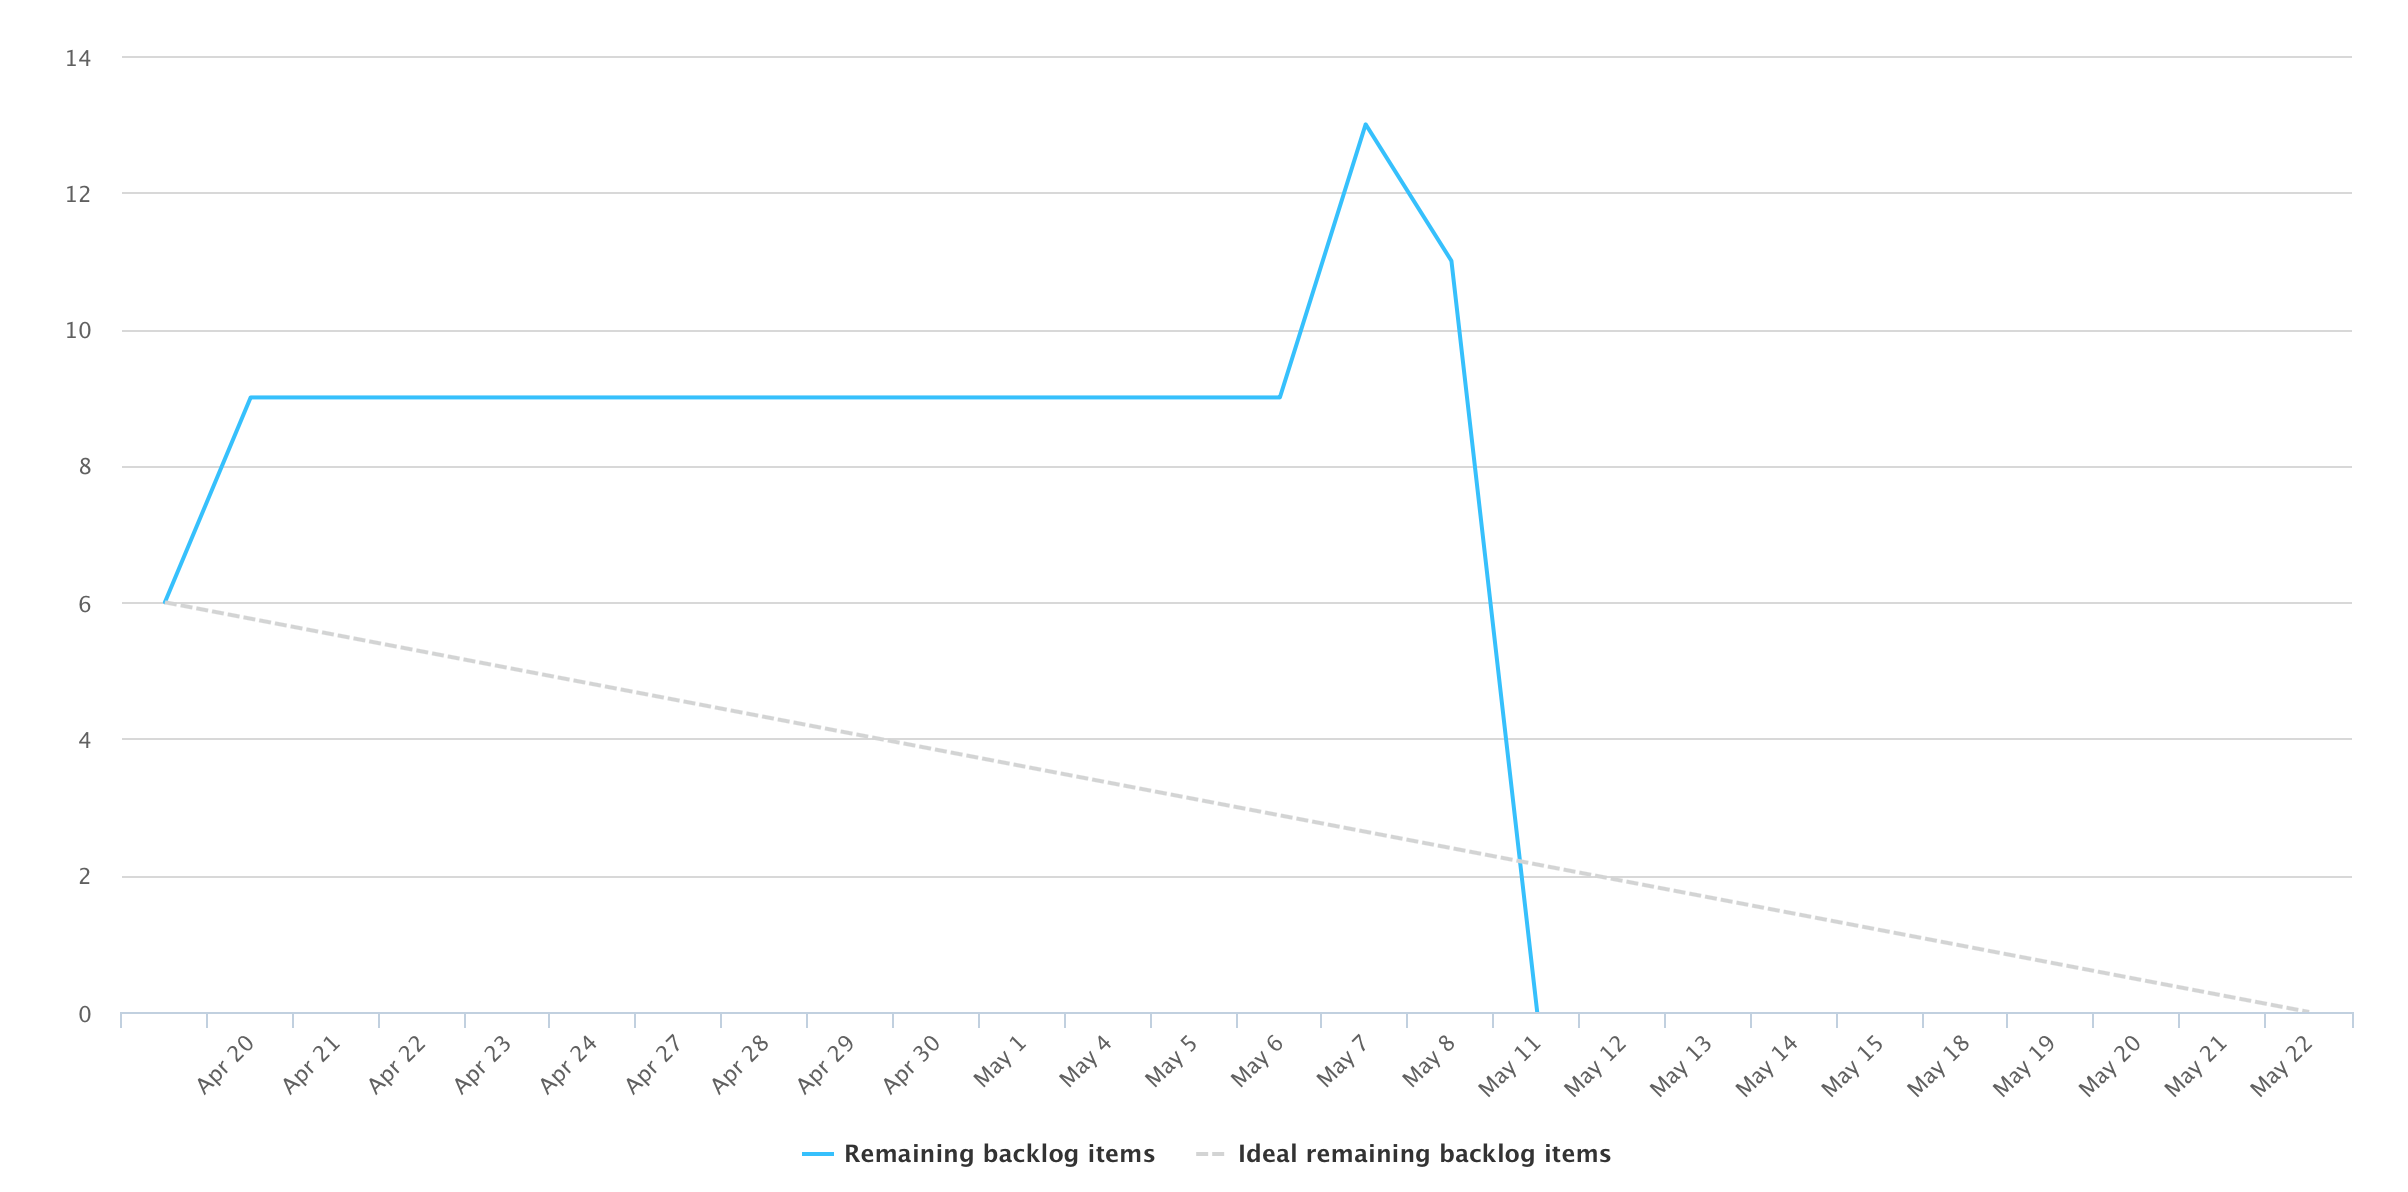
\includegraphics[width=1\textwidth]{./sprint1_burndown.png}}

Debido a que se utilizó una herramienta beta para administrar el proyecto, no se nos permitió ingresar una fecha de finalización del proyecto, siendo esta la designada por la misma. 



\newpage

\section{Comentarios}
El proyecto desarrollado solo cumple con los criterios pedidos por el Product Owner para la primera entrega, es decir, no se desarrolla de manera completa todos los stories definidos previamente. 
Es el caso de los resultados para cada campaña. El modelo diseñado para esta estapa es simple y no contempla todas las formas que puede presentar el objeto. En la medida de obtener mayor cantidad de casos posibles se podrá aprender más sobre la naturaleza del mismo y diseñarlo de forma completa. 
Lo mismo ocurre con el rol del docente y del personal de Secretaría o Dirección. En el desarrollo del código no se contempla la diferencia entre ambos, ya que no se implementan las restricciones para cada uno. Se toma como existencia un rol similar al del personal de la Secretaría o Dirección, ya que no tiene negado ningún tipo de acceso, pero se le asocia alumnos o padres como a un docente. 

En un comienzo se plantearon objetos a modelar que no eran necesarios, como sería el caso de la División. Se interpretó que la misma era necesaria para poder asociar un docente con un alumno y permitir así el acceso a este último. Luego de realizar diversas pruebas, de discutir al respecto y hablar con el Product Owner, se definió que no era necesario la implementación del mismo y se realiza una asociación directa desde el docente hacia el alumno. Se podrá observar más al respecto en la siguiente sección. 

Por otro lado, con referencia al seguimiento del proyecto con Scrum hubo errores. Se puede observar en el gráfico del Sprint la inconsistencia de su desarrollo. Esto ocurrió principalmente por haber agregado y eliminado tanto stories como tareas ya estando en la etapa de desarrollo. Se debería haber definido inicialmente, sin lugar a modificaciónes, todas las especificaciones por parte del cliente y las tareas que son requeridas para cada una. Luego de la reunión intermedia realizada con el Product Owner se agregaron nuevas tareas y se eliminaron otras, generando así un desorden en la organización de Scrum. Como equipo se debería mejorar la forma de desarrollar cada tarea, definiendo el effort y así las horas de manera más eficiente. De esta manera, al cargar las horas de trabajo por cada task, se podrá observar un comportamiento acorde. 


\newpage

\section{Diseño}
En primer lugar se presenta el diagrama de clases correspondiente a lo que luego se implementó para la primera demostración requerida por el Product Owner. Se decidió utilizar el lenguaje Python, debido a la experiencia por parte de los integrantes del proyecto, que permitiría avanzar de manera más rápida en la implementación del sistema. 

\centerline{\includegraphics[width=1.2\textwidth]{./diagramas/DiagramaDeClases.png}}

Se puede observar que el objeto Admin representará a los docentes y al personal de Secretaría o Dirección. Se decide no diferenciarlos para esta etapa del proyecto, ya que no es requerida la implementación de restricciones entre usuarios. Por el otro lado, se define que al los alumnos y los padres se los definirá a partir de Contact. Esta última clase se encarga de almacenar la información necesaria de un individuo. Será el objeto Agenda quien se encargue de agrupar a los mismos. De esta manera, en un futuro se podrá implementar de manera más sencilla la separación entre un alumno y un padre. 

El Clock está implementado a partir del patrón Observer. El mismo es utilizado para poder representar e implementar el paso del tiempo en el sistema. La bandeja de salida, denominada Scheduler, requiere del aviso del Clock para enviar ciertos mensajes. Los mensajes se encontrarán ordenados a partir de la fecha en la que el Admin determina que deben ser enviados. El objeto Observer, en este caso el Clock, se encargará de dar aviso del paso del tiempo para que los mensajes que fueron definidos con un tiempo menor, sean enviados.

Para poder definir de manera más clara ciertas situaciones desarrolladas en el esquema del diagrama de clases, se presenta a continuación diagramas de objetos. 

%\centerline{\includegraphics[width=0.8\textwidth]{./diagramas/}} 

%Describir brevemente el evento. 


Hablar sobre encapsulamiento y responsabilidades. "Existieron, a lo largo de la creación del diseño del sistema, situaciones en los que se definía un método para una clase y al implementarlo se notaba la asignación de responsabilidades a un objeto que no le correspondía. Este escenario se repitió reiteradas situaciones, corrigiéndose en el momento y adquiriéndose experiencia con respecto al comportamiento de los distintos objetos." %chamuyo mal, ni idea que poner..!!

















\end{document}